\chapter{呕 吐}

呕吐是人体的一种本能,可将食入胃内的有害物质吐出,从而起有利的保护性作用,但多数情况并非如此。频繁而剧烈的呕吐,可妨碍饮食,导致失水、电解质紊乱(如低钠、低钾血症)、酸碱平衡失调(幽门梗阻时常致代谢性碱中毒)、营养障碍,有时甚至发生食管贲门黏膜撕裂伤(Mallory-Weiss综合征)等并发症,对机体引起更多的有害后果。呕吐多伴有恶心的先兆,此时患者有欲吐的感觉,伴咽部或心窝部特殊的不适感,并常有头晕、流涎、心率减慢、血压降低等迷走神经兴奋症状。

呕吐首先须与食管性反流相区别。后者发生于食后一段期间,而无恶心的先兆,这是由于潴留于食管狭窄近端的扩张部或扩张的食管憩室中的食团,反流经口吐出,吐出物不含胃内容物。凡不伴恶心与呕吐协调动作者称为反胃。胃内容物经反胃进入口腔再行下咽者称为反刍,此两者应与呕吐加以区别。

呕吐中枢位于延髓。延髓有两个不同作用机制的呕吐机构:一是神经反射中枢-呕吐中枢,一是化学感受器触发区(chemoreceptor
trigger
zone,CTZ),接受引起呕吐的各种化学性刺激。呕吐中枢负责呕吐的实际动作,它接受来自消化道和其他躯体部分、大脑皮质、前庭器官以及化学感受器触发区的传入冲动。引起呕吐的大多数冲动,直接经由内脏传入神经至呕吐中枢,而非经由化学感受器触发区。在传入通路中,迷走神经纤维较交感神经纤维所起的作用更大,例如腹部的膨胀性冲动便可引起呕吐。主要传出通路为迷走神经(支配咽肌)、膈神经(支配膈肌)、脊神经(支配肋间肌、腹肌)以及迷走神经与交感神经的内脏传出神经(支配胃与食管),通过一系列复杂而协调的神经肌肉活动而引起呕吐。

化学感受器触发区本身不能直接引起呕吐的动作。此机构受兴奋时,发出对延髓呕吐中枢的传入冲动,然后引起呕吐动作。化学感受器触发区可受多种药物如吗啡、洋地黄、雌激素、氮芥等所兴奋。多巴胺是影响化学感受器触发区而导致呕吐的主要神经递质,而氯丙嗪、甲氧氯普胺(胃复安)、多潘立酮(吗丁啉)为多巴胺受体阻滞剂,因而具有镇吐的作用。呕吐在诊断和鉴别诊断上须注意下列各项检查:

问诊:详细了解呕吐有无伴恶心的先兆,和食物、药物、体位、精神因素等的关系,有无酗酒史以及以往类似的发作史。呕吐时间和进食时间的关系。呕吐物的质和量,呕吐的伴随症状。腹部疾病或腹部手术史,颅脑疾病或外伤史,过敏史或放射治疗史,以及高血压、心脏病、肾脏病、糖尿病与内分泌疾病病史。生育期妇女要询问月经史。

细菌性食物中毒有不洁饮食史。急性中毒有误服有关毒物的历史。晨间呕吐多见于妊娠呕吐。颅内肿瘤的特点为不伴有恶心的喷射性呕吐,和饮食无关,吐后头痛可暂时缓解;在第四脑室肿瘤时,呕吐更为严重和频繁。呕吐量大、呈喷射性者,常见于幽门狭窄合并胃扩张与潴留。呕吐物含大量胆汁者,说明有胆汁逆流入胃,常为较顽固的呕吐,可见于高位小肠梗阻、胆囊炎、胆石症,有时也见于妊娠剧吐、晕动病等。呕吐物带粪臭气者,常见于小肠下段的肠梗阻。吐泻交替发作者,须注意细菌性食物中毒、霍乱或副霍乱、过敏、急性中毒等。呕吐伴高热者,须注意急性感染。呕吐伴剧烈头痛者,须注意颅内高压症、青光眼等。呕吐伴耳鸣、眩晕者,须注意迷路疾患、晕动病。

体格检查:先着重腹部检查。注意腹部外形、胃肠蠕动波与肠型、腹部压痛与反跳痛、腹块、腹水征、肠鸣音、振水音等。有指征时作神经系统、前庭神经功能与眼科检查等。

实验室检查:有指征时作尿糖、尿酮体,血、尿常规,血糖,血清钾、钠、氯、钙、淀粉酶、二氧化碳结合力,甲状腺、甲状旁腺功能测定,血pH,尿妊娠试验,肝、肾功能,脑脊液常规,呕吐物的检查,疑有化学或药物中毒时作毒理学分析等。

特殊器械检查:有指征时作腹部B超、腹部透视或平片,颈椎摄片、胃肠钡餐透视,消化道碘水造影,胃十二指肠镜检查,心电图、眼科检查,脑电图、CT或脑磁共振显像,脑血管造影等。

呕吐的原因相当繁多,一般原因如表\ref{tab20-1}所示。

\begin{table}[htbp]
\centering
\caption{呕吐的一般病因}
\label{tab20-1}
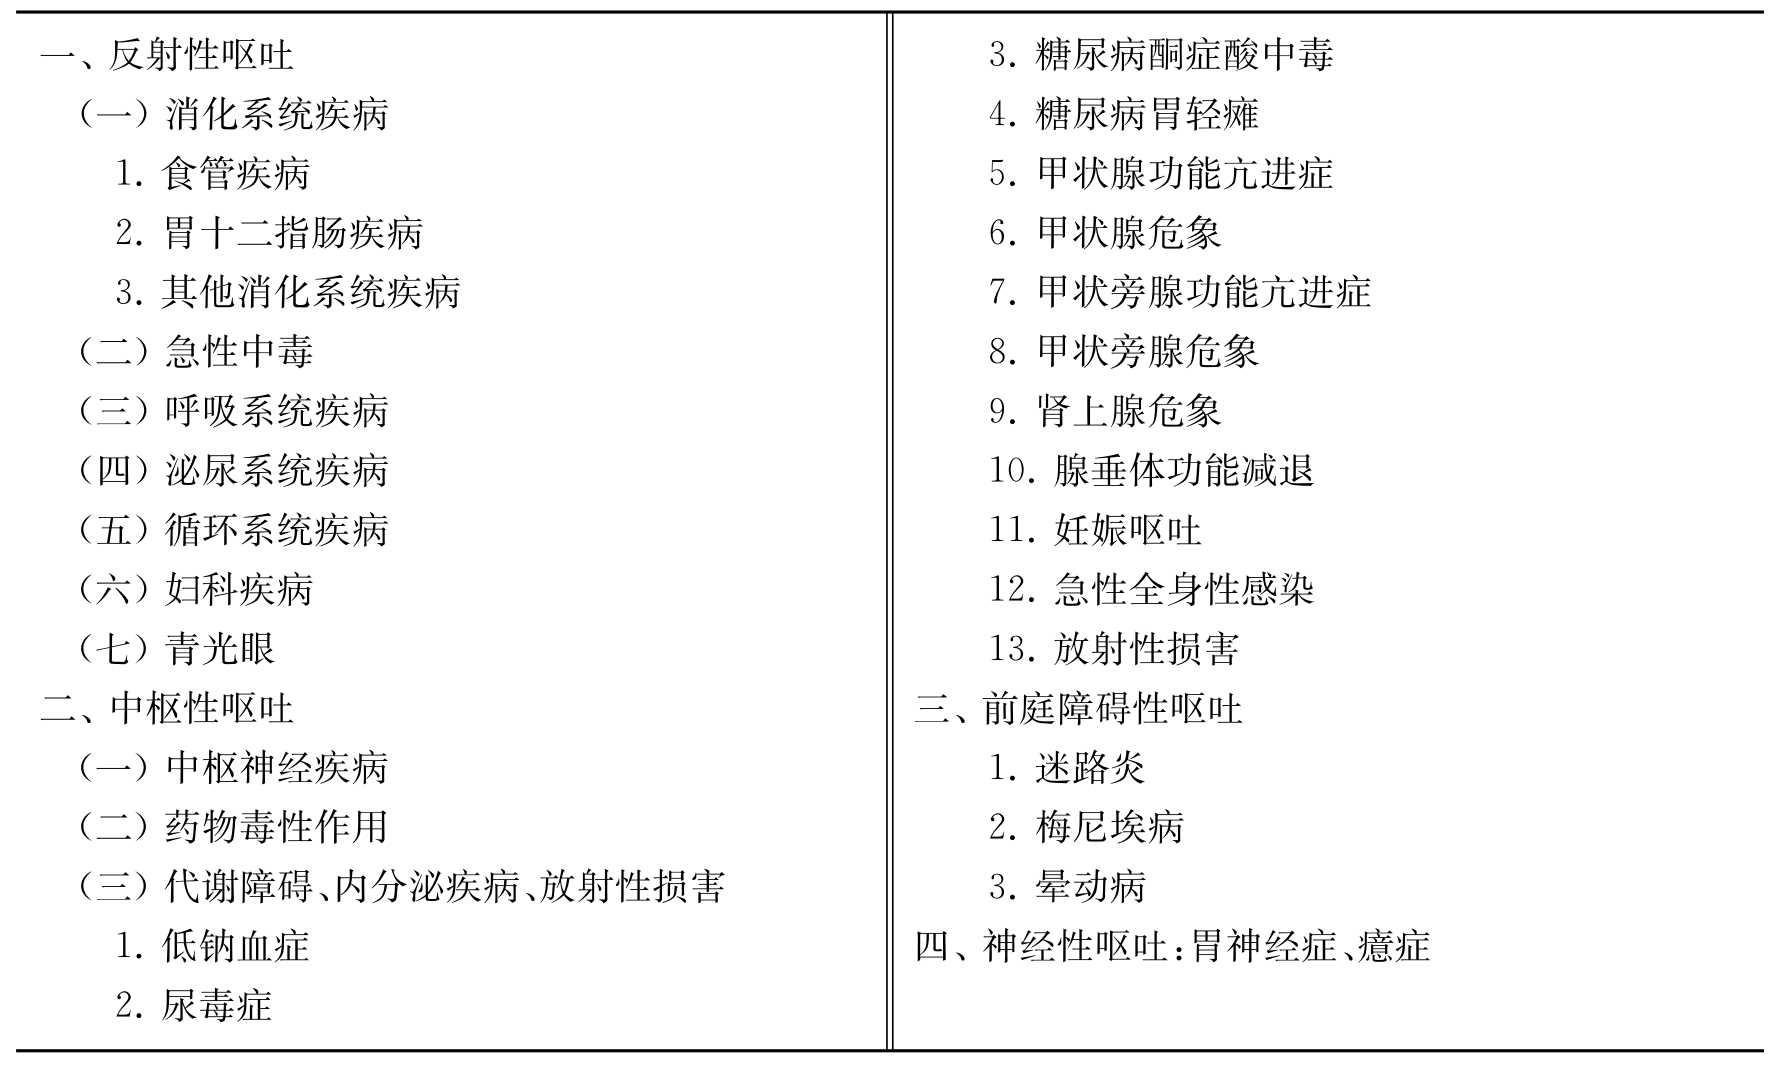
\includegraphics[width=5.89583in,height=3.5625in]{./images/Image00120.jpg}
\end{table}

\protect\hypertarget{text00161.html}{}{}

\section{63 反射性呕吐}

\subsection{一、消化系统疾病}

\subsubsection{(一)食管疾病}

除了食管炎如腐蚀性食管炎可引起呕吐外,还有:

\paragraph{1.食管黏膜剥脱症}

多发生于健康人,大多数患者有明显诱因,如快速吞咽干硬、粗糙、热烫食物或误吞鱼刺、枣核、骨性异物,使食管黏膜受到急性物理性损伤,恶心、呕吐可能成为食管黏膜剥脱的始动力,造成食管内压升高,食管黏膜上皮层与固有层之间分离加剧,两层之间血管出现断裂、出血甚至形成黏膜下血肿,最后导致食管黏膜表层断裂并与固有层完全分离,灰白色条带膜状物可吐出口外。患者除有恶心呕吐外,还可有消化道出血、胸骨后痛、吞咽时疼痛加剧,严重时伴吞咽困难。

胃镜检查是诊断食管黏膜剥脱症的必要手段。内镜下可见食管黏膜纵行条索状肿胀、隆起、剥脱,甚至游离于食管腔内,色泽灰白或呈暗紫红色。

\paragraph{2.自发性食管破裂}

常发生于呕吐、咳嗽后,少数无明显诱因,多见于中老年男性,破口部位多数在食管中下段。患者表现为呼吸困难、持续胸痛,少数可出现发热、皮下气肿。胸片、CT可发现胸腔积液,食管造影可发现造影剂外溢,胸腔引流出食物残渣可确定诊断。对此少见疾病,内科医生尤其要注意鉴别。

\subsubsection{(二)胃十二指肠疾病}

胃十二指肠疾病所致的呕吐较为多见,常有恶心的先兆,吐后常感到轻松。吐出物为咽下的食物、胃液、胆汁等,也可含有血液或为纯血(呕血)。

\paragraph{1.胃黏膜刺激或炎症}

胃黏膜受刺激或急性胃(肠)炎或慢性胃炎的急性发作时,均可引起恶心、呕吐。病因可为:①细菌性,如细菌性食物中毒(参见第73.1节);②化学性,如某些化学物品(如烈酒)或药物(如阿司匹林、磺胺类、氨茶碱、抗生素、化疗药物等)的刺激;③物理性,如胃过度充盈时对胃黏膜的直接刺激。药物、食物过敏所致呕吐常与个体耐受性有关。

嗜酸性粒细胞性胃肠炎(eosinophilic
gastroenteritis,EG)是一种以胃肠道某些部位局限性或弥漫性嗜酸性粒细胞浸润为特征的疾病,病变可累及全消化道各层。可分为:①黏膜病变型:黏膜内大量嗜酸性粒细胞浸润,以恶心、呕吐、腹痛、腹胀等为主要表现;②肌层病变型:浸润以肌层为主,以幽门或小肠梗阻为主要表现;③浆膜病变型:主要累及浆膜,多表现为腹水。EG患者上述三型可单独或同时出现,临床上黏膜型最多见,其诊断标准为:①有腹痛、腹泻、恶心、呕吐等症状;②消化道活检或腹水检查有嗜酸性粒细胞浸润;③除外继发性疾病引起的胃肠道EOS浸润,如寄生虫感染、风湿病,该病极易误诊,因此对有消化系统症状者,注意询问过敏史,重视血及腹水的EOS计数,必要时重复检查、人工计数;对常规抑酸等治疗效果不佳时,注意复查胃肠镜,多部位活检,请病理医生认真阅片。

\paragraph{2.各种原因的幽门梗阻}

幽门梗阻所致呕吐常呈周期性发作,于食后一段时间出现,可呈喷射性。病因为消化性溃疡、胃癌、胃黏膜脱垂症、胃肉芽肿(嗜酸性或血吸虫病引起)、异位胰腺以及罕见的胃肿瘤等。梗阻可能由于:①幽门括约肌痉挛,多发生于消化性溃疡、胃癌,患者多为中年或中年以上,伴有或不伴有幽门管黏膜充血与水肿,而单纯性幽门括约肌痉挛所致的梗阻少见;②幽门管瘢痕性狭窄,一般由消化性溃疡引起,常不致引起完全性梗阻;③幽门管被肿瘤、脱垂的胃黏膜、异位胰腺或肉芽肿所梗阻。

幽门痉挛所致呕吐通常在进食后几小时内发生,痉挛可在解痉剂注射之后缓解,胃排空障碍得以解除,呕吐也停止,这种情况可见于消化性溃疡活动期与慢性胃炎急性发作时。幽门器质性狭窄所致的呕吐,常并发胃扩张与胃潴留,常在食后6~12小时左右发生,有时呈喷射性,呕吐量大,甚至含有隔宿的食物。器质性狭窄大多由于溃疡病瘢痕狭窄引起,发病多在中年,呕吐物中不含胆汁;少数由胃癌引起,发病多在中年以上,少部分胃癌浸润胃体、胃窦甚至全胃(皮革胃)致胃蠕动减少,虽无幽门梗阻,也可有呕吐、腹胀表现。由于罕见的胃肿瘤(肉瘤、淋巴肉瘤、霍奇金淋巴瘤等)、胃肉芽肿等引起者更为少见。

胃黏膜脱垂症时,脱垂的胃黏膜可阻塞幽门,并可继发脱垂胃黏膜的发炎、糜烂与溃疡形成,引起间歇性上腹痛、恶心、呕吐,甚至上消化道出血,临床上需与消化性溃疡相鉴别。胃镜检查可明确诊断。

\paragraph{3.功能性消化不良}

主要表现为慢性持续或复发性中上腹痛或不适,有时可伴恶心、呕吐。功能性消化不良的诊断参见第81.2节。

\paragraph{4.肠系膜上动脉综合征}

本综合征并非少见。发病以体型瘦长的女性为多,罹患年龄多在20~40岁。任何原因导致肠系膜上动脉与腹主动脉之间的距离变小,致夹在其中的十二指肠受压而造成排空困难,即可产生本综合征的病象。主要表现为逐渐发生的上腹胀痛、恶心与呕吐,于食后数小时或更短时间发作,采取俯卧位或左侧卧位时可使症状缓解。X线钡餐透视检查可见十二指肠近段扩张,钡剂淤滞,胃与十二指肠排空延缓,十二指肠水平段与上升段交界处压迫征象可见典型“笔杆征”。通过放射科医生多体位反复观察可减少漏诊本症。

\paragraph{5.输出袢综合征}

本综合征以周期性大量胆汁性呕吐为临床特征,由于部分胃切除术后空肠输出袢的功能性梗阻引起,发生原理未明。典型症状常于手术后第8~12天出现,表现为上腹部饱胀或胀痛,特别在食后,伴恶心、呕吐。呕吐后或插入胃管抽空胃内容物后症状缓解,但几小时后症状又可再现。X线钡餐透视检查显示胃内有大量空肠滞留液。多数病例经对症治疗后症状缓解。由于手术瘢痕收缩、手术误差等引起的空肠输出袢器质性狭窄,如反复出现机械性肠梗阻的表现,则往往需手术治疗。

\paragraph{6.其他原因的十二指肠梗阻}

十二指肠梗阻可因肠外病变压迫或肠内病变阻塞所引起,表现为十二指肠病变部位肠腔的局限性狭窄及其上部的肠段扩张,最常见的症状是间歇性腹痛与呕吐。腹痛多位于上腹正中或偏右,可为间歇性隐痛乃至阵发性剧痛,伴恶心、呕吐,有时呕血与便血。上腹部可出现蠕动波、振水音,有时出现腹部包块。

十二指肠癌少见,易漏诊,内镜检查是诊断本病的主要手段。患者常有不同程度的呕吐、纳差、消瘦、腹胀、腹痛、消化道出血。

其他原因所致的十二指肠梗阻,如非特异性炎症性粘连或肠腔狭窄、隔膜畸形、环状胰、肉瘤、肉芽肿性变等均少见,诊断须根据X线钡餐检查、十二指肠镜检查与剖腹探查。近年小肠镜的应用对本病的诊断有很大的帮助。胃十二指肠克罗恩病(CD)少见,临床上极易漏诊或误诊。其临床表现无特殊,可有恶心、呕吐、腹痛、腹胀、上消化道出血,累及胃窦、十二指肠,内镜表现为反复发作或不易愈合的溃疡,临床上可有幽门梗阻及十二指肠梗阻的症状。对于胃或十二指肠溃疡,特别是年轻且伴有幽门梗阻的患者,常规抗溃疡治疗效果不佳时,要考虑胃及(或)十二指肠CD的可能,做超声内镜和腹部CT检查,在保证安全的前提下,内镜下深取活检或黏膜下层切除活检。对有手术指征患者,可行外科手术治疗并可明确诊断。

\subsubsection{(三)其他消化系统疾病}

\paragraph{1.腹腔脏器急性炎症}

急性腹膜炎早期呕吐轻微而时发时止,但病情发展时则呕吐成为持续性,早期的呕吐为反射性,继之则为中毒性,最后则由于麻痹性肠梗阻所引起。急性阑尾炎早期常有脐周或中上腹痛,伴恶心、呕吐与纳差,易被误诊为急性胃炎。急性胆囊炎、胆石绞痛及胆道蛔虫病,也常常有恶心、呕吐,但多不严重,呕吐物可为食物、胃液、胆汁,有时可见蛔虫(不仅可见于胆道蛔虫病,也可见于肠道蛔虫病),呕吐后病情未见减轻。急性胰腺炎也常常有恶心、呕吐,但多不严重,常有上腹部持续性疼痛并可向腰背部放射,进食后可加重。由于呕吐并非上述疾病的主要表现,诊断参见第78.1节。

\paragraph{2.急性病毒性肝炎}

本病可有纳差、乏力、厌油、恶心、呕吐、腹痛,可误诊为急性胃炎、消化不良等;如急性肝炎病情加剧,重新出现呕吐,黄疸加深,须考虑急性或亚急性重症肝炎的可能性。

\paragraph{3.肠梗阻}

本病的主要症状是呕吐、肠绞痛与停止排便排气。呕吐常剧烈,并伴恶心。早期的呕吐为神经反射性,呕吐物初为食物、胃液,继而为黄绿色的胆汁。反射性呕吐停止后,隔一段时间而出现典型肠梗阻的反流性呕吐。两种呕吐间隔时间的长短,取决于梗阻部位的高低。梗阻部位愈高,间隔时间愈短。低位回肠梗阻时,时间间隔较长。反流性呕吐是由于肠内积液不能通过梗阻部位,积聚于梗阻上部的肠段,达到相当大量时形成肠逆蠕动而吐出所致。呕吐物早期呈胆汁样液体,继而呈棕色或浅绿色,晚期呈较稠厚而带粪臭气的液体,这是由于食物在低位肠道内有较长时间的潴留,受肠内细菌作用而腐败分解所致。病因可为肿瘤、炎症、先天性畸形、结石、大块食物、肠扭转、肠套叠等。

肠旋转不良临床少见,多发生于小儿,成人偶可见到。因肠的位置先天异常,造成肠扭曲、压迫、粘连而导致肠梗阻,常需剖腹探查确立诊断。

\paragraph{4.假性肠梗阻}

假性肠梗阻(intestinal pseudo
obstruction,IPO)是由于肠道肌肉神经病变引起的肠道运动障碍性疾病。具有反复发作的肠梗阻症状及体征,而无肠内外机械性肠梗阻因素存在的一种综合征。根据病变部位不同,分为小肠假性梗阻和结肠假性梗阻;根据病程不同,可分为急性和慢性梗阻。根据病因可分为原发亦可继发于结缔组织病,如系统性红斑狼疮、皮肌炎、干燥综合征、未分化结缔组织病,继发性IPO还可出现肾盂输尿管积水、腹水、血液等其他系统受累,并且多见于女性。小肠假性梗阻因小肠动力低下肠内容物通过缓慢,肠腔扩张达到一定程度,可产生肠梗阻的临床表现,如腹胀、呕吐。腹部平片、腹部CT、小肠镜、小肠测压和小肠通过时间测定有助于诊断。如剖腹探查,病理检查注意有无肌间神经丛病变。临床上对原因不明的IPO,尤其是女性,需注意有无腹水、肾脏、血液等系统受累,尽早行免疫学检查,排除风湿疾病,以期早期诊断,并避免不必要的外科手术。

\subsection{二、急性中毒}

参见第74节。

\subsection{三、呼吸系统疾病}

急性肺炎在发病初期可有呕吐,小儿尤多见。百日咳的痉挛期,在痉挛性咳嗽发作之后,常有反射性呕吐,将胃内食物全部吐出。急性扁桃体炎因细菌毒素刺激,患者可呕吐胃内容物,小儿尤多见。

\subsection{四、泌尿系统疾病}

急性肾炎的高血压脑病,呕吐常突然发生(中枢性呕吐)。急性肾盂肾炎以恶心呕吐而起病者约占30\%~36\%,特别是在女性。肾结石绞痛发作,呕吐多与绞痛同时出现。

\subsection{五、循环系统疾病}

急性心肌梗死的早期,特别是当疼痛剧烈时,常发生恶心、呕吐,可能由于心肌病灶的刺激引起迷走神经对胃肠的反射性作用所致。偶尔疼痛定位于上腹部而呕吐剧烈者,可被误诊为急性胃炎或其他急腹症。少数以恶心、呕吐为主要症状的心梗尤要注意鉴别。主动脉夹层动脉瘤破裂也可引起上腹痛与呕吐,甚至猝死。

充血性心力衰竭有时发生呕吐,可能与肝淤血有关,但在洋地黄治疗时还须警惕洋地黄的毒性作用所致。

在低血压伴昏厥或休克的初期,也常有恶心、呕吐,伴苍白、心悸、出冷汗等自主神经失调症状。

\subsection{六、妇科疾病}

妇女内生殖器官的急性炎症(急性附件炎等)时,炎症刺激经由自主神经的传入纤维,将冲动传入呕吐中枢而引起反射性呕吐。炎症扩散则引起急性盆腔腹膜炎,出现高热、下腹痛与压痛、白细胞增多,并有腹胀、鼓肠、便秘、排尿困难等症状。宫外孕破裂、卵巢囊肿扭转也可有呕吐,但还有腹痛、休克、尿路刺激症、腹泻以及阴道后穹隆穿刺出不凝血等表现。

\subsection{七、青光眼}

闭角型青光眼是原发性青光眼较常见的一种类型,患者以女性为多,发病多在40岁以后。患者头痛常剧烈,可因眼压增高,经三叉神经的反射作用而引起呕吐。有时可因忽略眼科检查而被误诊为内科疾病。

\protect\hypertarget{text00162.html}{}{}

\section{64 中枢性呕吐}

\subsection{一、中枢神经系统疾病}

\subsubsection{(一)脑血管病变}

高血压脑病时,由于血压急剧升高,脑血液循环急剧障碍,导致脑水肿与颅内压力升高,出现剧烈头痛、眩晕、恶心、呕吐,甚至惊厥、昏迷等症状。

高血压动脉硬化症患者突然发生剧烈头痛与呕吐,须警惕脑出血的发生。

脑出血,特别是小脑出血,常出现剧烈头痛、呕吐。呕吐是由于出血穿透第四脑室,或血肿压迫第四脑室、直接刺激呕吐中枢所致。以暴发性后脑部疼痛、呕吐为前驱症状,继而出现脑膜刺激征,脑脊液呈血性者,可诊断为蛛网膜下腔出血。Wallenberg综合征发病通常在40岁以上,病变主要由于椎动脉血栓闭塞引起,有眩晕、恶心、呕吐等前庭神经刺激症状(参见第158节)。

椎-基底动脉供血不足大多发生于中年以上,男性发病高于女性一倍以上。临床表现多种多样,最常见者为眩晕,或伴恶心、呕吐,提示前庭功能障碍(参见第158节)。

\subsubsection{(二)中枢神经感染}

颅内感染可因炎症性渗出导致颅内压增高,而有头痛、呕吐等症状。乙型脑炎大多累及小儿,常有恶心呕吐,多发生于病程第1~2天,呕吐次数不多,仅少数呈喷射性,如不注意可诊断为急性胃炎。其他原因的病毒性(脑膜)脑炎发生恶心呕吐者也不少见,诊断参照流行病学史、临床表现与有关的病毒学、脑脊液检查。

脊髓灰质炎的前驱期与麻痹前期,也常有头痛、咽痛、恶心、呕吐,与流行性感冒相似。流行性脑脊髓膜炎常以高热、寒战、头痛、恶心、呕吐急性起病,呕吐是由于颅内压增高、呕吐中枢受刺激,以及脑膜受刺激而产生的反射性作用引起,在本病流行期间不难确定诊断。结核性脑膜炎或真菌性脑膜炎并非罕见,遇不明原因发热、头痛、呕吐的病例要提高警惕。

脑脓肿常为继发性,大多由于邻近化脓性病灶的直接蔓延,例如耳源性脑脓肿,起源于慢性化脓性中耳炎或乳突炎;少数病例则起源于血行性或外伤性感染。耳源性脑脓肿多位于颞叶或小脑,多为单发性。血行性脑脓肿常为多发性。如有颅内压增高及(或)脓肿直接刺激呕吐中枢时,则除感染症状之外,还有头痛、呕吐等症状。

脊髓痨是晚期神经梅毒,当发生胃危象时,有闪电样痉挛性胃痛、呕吐等症状。艾滋病侵犯神经也可有类似表现,临床上需注意排除。

\subsubsection{(三)偏头痛}

本病以阵发性半侧头痛为临床特征,女性罹患较多,多于青春期开始,至中年或闭经后自行停止。病因未明。30岁以前起病者多有遗传性。精神刺激、妊娠、饮酒、吸烟等均可为发病诱因。发作前常有乏力、嗜睡或烦躁不安等症状,头痛前常有同侧偏盲、眼前闪动性光点和颜面感觉异常等前驱症状。头痛剧烈时出现恶心、呕吐,吐后头痛减轻。麦角制剂治疗可使症状迅速缓解(参见第154节)。

\subsubsection{(四)脑肿瘤}

脑肿瘤常有三种主要症状:①呕吐;②头痛;③视力障碍,眼底检查常见有视乳头淤血。此外还常有不同程度颅神经损害的症状等。呕吐原因由于:①肿瘤发生在脑脊液通路或其附近,引起颅内压迅速增高;②肿瘤直接压迫和刺激延髓呕吐中枢,或前庭神经、迷走神经等。幕下脑瘤引起呕吐者较幕上脑瘤早而多见。脑肿瘤所致的呕吐,和饮食关系不大,常发生于头痛剧烈之时,呕吐后头痛可暂时减轻。无明显消化系疾病的顽固性呕吐,须考虑颅内尤其是脑室占位性变的可能性。早期脑瘤常易被误诊为神经症。小儿脑瘤患者,往往表现为不伴有头痛的喷射性呕吐。CT、MRI对诊断帮助最大。

\subsubsection{(五)脑畸形性疾病}

脑积水常由于脑脊液循环阻塞所引起,以脑室扩张与脑脊液量增多为特征。发生原理由于:①脑脊液循环通路受阻;②脑脊液吸收的缺陷;③脑脊液产生过多。由此引起一系列颅内压增高所致的症状,如头痛、呕吐、视力障碍、视乳头水肿等。成年人脑积水由于骨缝已闭合,常于早期即出现上述症状。脑超声检查、头颅平片、CT、MRI等常有助于诊断。

\subsubsection{(六)癫痫}

极少部分癫痫患者表现为自主神经症状的发作,包括上腹疼痛不适、呕吐、出汗、面色潮红、苍白、瞳孔散大等,个别患者以呕吐表现为主,既往曾称之为呕吐型癫痫。其特征为:①长期反复呕吐无诱因;②呕吐常突然发作,呈阵发性发作,严重时一天多次;③无消化系统器质性病变;④脑电图有异常;⑤抗癫痫药治疗有效。

\subsubsection{(七)头部外伤}

脑震荡之后,如意识障碍在6小时内消失,则可出现头痛、呕吐、眩晕,这并非脑有器质性损伤,而是呕吐中枢受物理刺激所致。

脑挫裂伤常引起明显的头痛、呕吐。持续性剧烈头痛伴喷射性呕吐与意识障碍加重者,须考虑有颅内血肿形成。

\subsection{二、药物毒性作用}

吗啡、洋地黄、雌激素、甲睾酮等,以及氮芥、环磷酰胺、丙卡巴肼、氟尿嘧啶、丝裂霉素C等化疗药物,均可兴奋化学感受器触发区,引起呕吐。

洋地黄疗程中最早的中毒症状常是纳差、恶心、呕吐,如兼有心律失常,更可肯定洋地黄中毒的诊断。

\subsection{三、代谢障碍、内分泌疾病、放射性损害}

\subsubsection{(一)低钠血症}

重度低钠性失水患者常有乏力、恶心、呕吐、肌肉痉挛、腹痛等症状,甚至神志淡漠、嗜睡、血压下降与昏迷。病因多为急性胃肠炎、大面积烧伤、肾上腺危象、糖尿病酮症酸中毒、失盐性肾炎等。

稀释性低钠血症(如水中毒、抗利尿激素分泌异常症)也常引起频繁呕吐。

\subsubsection{(二)尿毒症}

尿毒症患者常较早出现头痛、恶心、呕吐。如并发尿毒症性胃炎,则呕吐更为严重。有一些患者因为恶心呕吐验血检查肾功能而诊断患尿毒症。

\subsubsection{(三)糖尿病酮症酸中毒}

糖尿病酮中毒的诱因多为感染、创伤、手术、麻醉、中断胰岛素治疗等,患者常以厌食、恶心、呕吐等为早期症状。由于厌食、呕吐与多尿,致加重了失水与失钠,又使呕吐加剧,促进酮症性昏迷。

\subsubsection{(四)糖尿病胃轻瘫(diabetic gastroparesis,DGP)}

DGP是糖尿病常见并发症,发生率达50\%~76\%,主要表现为胃排空延迟,临床可见厌食、恶心、呕吐、早饱、腹胀等症状,严重影响患者的生活质量。DGP的诊断标准为:①糖尿病史;②存在持续性早饱、腹胀、厌食、恶心、呕吐等临床症状;③内镜和钡餐检查排除机械性梗阻;④放射性核素标记试验、胃排空试验、实时B超、胃压测定术、胃电图提示胃排空延迟,大部分学者认为糖尿病患者在高血糖基础上可致内脏的自主神经病变、胃肠激素异常及微血管病变,使胃张力减弱和运动减慢。

\subsubsection{(五)甲状腺功能亢进症(甲亢)}

甲亢的临床表现错综复杂,典型者表现在消化系统为多食易饥、体重下降、大便次数增多,严重者有肝功能异常。以顽固性呕吐为突出表现者临床较少见,极易误诊、漏诊。老年甲亢患者以厌食、恶心、呕吐、消瘦为突出表现者稍多。对无明显诱因的呕吐,排除消化系统和中枢神经系统疾病后,注意有无心率增快,即使无甲状腺肿大、甲状腺无震颤及血管杂音,即使为妊娠期女性,也应及早行甲状腺功能检查,以确定是否有甲亢。

\subsubsection{(六)甲状腺危象}

本症是甲状腺功能亢进症的严重并发症,诱因为感染、创伤、未经充分准备而施行手术、精神刺激等,\textsuperscript{131}
I治疗甲状腺功能亢进症时也偶尔诱发。主要症状为高热或过高热、心动过速、不安或谵妄、大汗、呕吐与腹泻等,如不及时救治,可因周围循环衰竭而引起死亡。

\subsubsection{(七)甲状旁腺功能亢进症}

原发性甲旁亢临床少见,主要临床表现有骨痛、关节痛、泌尿系结石表现,胃肠道症状有恶心、呕吐、腹胀、食欲下降、便秘,甚至有消化性溃疡,也可出现消瘦、乏力、贫血、血沉增快。故临床上对不明原因呕吐、腹胀、便秘、食欲下降患者,注意患者是否有骨痛或骨质改变及泌尿系结石,检查血钙、磷、尿钙、血清甲状旁腺素,进一步可行甲状旁腺超声、CT或ECT检查,以明确甲旁亢的诊断。

\subsubsection{(八)甲状旁腺危象}

甲状旁腺功能亢进症在应激情况下当血清钙增高至13mg/dl以上时,即可产生甲状旁腺危象(高血钙危象),临床表现为口渴、多尿、厌食、乏力、恶心、呕吐、便秘、肌肉软弱等症状。严重者发生昏迷与死亡。应立即补充生理盐水,注意电解质及酸碱平衡,注射降钙素,必要时予血液透析。

\subsubsection{(九)肾上腺危象}

慢性肾上腺皮质功能减退症(艾迪生病)可因感染、创伤、手术、过度劳累、中断糖皮质激素治疗等而诱发危象(肾上腺危象)。主要临床表现为体温降低、恶心、呕吐、失水、血压下降与周围循环衰竭,最后可陷入昏迷。由于患者常有吐泻发作,可被误诊为急性胃肠炎。

\subsubsection{(十)腺垂体功能减退症}

是由部分或全部垂体前叶被破坏,而产生单一或多种内分泌靶腺功能继发性减退的疾病,如性腺、甲状腺、肾上腺。除不明原因的恶心、呕吐外,还有性欲减退、阴毛脱落、精神萎靡、反应迟钝、怕冷、贫血、闭经、低血糖、低血压、皮肤干燥、心率慢等临床表现。测定皮质醇、甲状腺、性激素以及垂体MRI可明确诊断。及时补充皮质激素等靶腺激素,可防止垂体危象的发生。

\subsubsection{(十一)妊娠呕吐}

素来健康的已婚生育期妇女,忽于清晨起床后呕吐,连续多天,须注意妊娠呕吐。妊娠呕吐约见于半数的孕妇,多发生于妊娠期5~6周左右,但最早可见于妊娠第2周,一般持续数周而消失。发生原理未明,有认为与血中雌激素水平增高有关,精神因素可起一定的作用。患者常有困倦、思睡,嗜食酸味的食品。呕吐之前常有恶心。呕吐与精神因素有一定的关系,分散患者的注意力可使呕吐减轻。体检乳头颜色加深。尿液妊娠试验反应阳性。症状轻重各有不同。轻症者不影响日常生活与健康,称妊娠呕吐。重症者可引起失水、电解质紊乱、酸碱平衡失调、营养障碍,则称为妊娠剧吐。

妊娠毒血症发生于妊娠期第24周以后,多见于年轻初产妇,主要症状为血压升高、蛋白尿、水肿与视力减退,恶心与呕吐常是先兆子痫的表现。

\subsubsection{(十二)急性全身性感染}

许多急性全身性感染性疾病,可发生恶心、呕吐,尤以重症病例。可能由于发热与毒血症状态时,胃蠕动与胃分泌减少,消化功能减退,未消化的食物易积存于胃内,并易于呕出。儿童的呕吐中枢兴奋阈限低,在急性传染病时尤易发生呕吐。

最常引起呕吐的急性感染,首先是中枢神经急性感染、胃肠道急性感染、腹腔脏器的急性感染、泌尿系感染等。病原体可为细菌性、病毒性、真菌性、疟原虫等。细菌性食物中毒时,呕吐多发生于腹泻之前;霍乱与副霍乱时,呕吐多发生在腹泻之后。近年艾滋病的发病呈上升趋势,临床有艾滋病引起呕吐的报道,需要我们高度警惕。

\subsubsection{(十三)放射性损害}

在深部X线治疗,镭照射治疗、钴照射治疗等之后,均可发生食欲减退、恶心、呕吐。急性放射病的初期表现为神经系统的过度反应,致出现头晕、头痛、乏力、恶心、呕吐、腹泻等症状。

\protect\hypertarget{text00163.html}{}{}

\section{65 前庭障碍性呕吐}

\subsection{一、迷路炎}

本病是急性与慢性化脓性中耳炎的常见并发症,临床病理学上可区分为迷路周围炎、局限性迷路炎、弥漫性浆液性迷路炎与弥漫性化脓性迷路炎四种类型,而后者的病情最严重。主要临床表现为发作性眩晕、恶心、呕吐、眼球震颤等,诊断主要根据病史与耳科检查。

\subsection{二、梅尼埃病}

本病以男性罹患较多,发病多在中年。典型表现为突然发作的旋转性眩晕(多为水平性)、耳聋与耳鸣。眩晕发作时意识清醒,常伴有面色苍白、出冷汗、恶心、呕吐、血压下降等反射性迷走神经刺激症状。发作历时数分钟乃至数小时以上,间歇期也各有不同(参见第157节)。

\subsection{三、晕动病}

本病症状发生在航空、乘船、乘汽车或火车时,以苍白、出汗、流涎、恶心、呕吐等为主要的表现。原因未充分明了。由于反复的俯仰运动、旋转、或上下颠簸所致的迷路刺激,明显地起重要的作用。迷路功能丧失的人常不致罹患晕动病。遗传和精神因素可能有重要关系。有些身体健康的人对乘车乘船完全不耐受,有的虽能耐受乘船乘车,但在车船中嗅到不愉快的气味或听到震耳的噪音等不良刺激,即可发生恶心、呕吐。

\protect\hypertarget{text00164.html}{}{}

\section{66 神经性呕吐}

呕吐可为胃神经症或癔症症状之一。其特点是呕吐发作和精神刺激有密切的关系。呕吐可于食后立即发生,呕吐全不费力,每口吐出量不多,吐毕又可再食,虽长期反复发作而营养状态影响不大。嗅到不愉快的气味、听到震耳的噪音、或见到厌恶的食物而出现的呕吐,称条件反射性呕吐,也属神经官能性呕吐范畴。对神经官能性呕吐须小心除外一切器质性病因方能确定诊断。女性和神经不稳定的人,其呕吐中枢兴奋阈限较低,受各种刺激作用时易发生呕吐。

\protect\hypertarget{text00165.html}{}{}

\section{参考文献}

1.陈元芳.恶心呕吐.//潘国宗,曹世植.现代胃肠病学.北京:科学出版社.1994

2.唐光佐,等.肠系膜上动脉综合征.中华外科杂志,1982,20:476

3.张铁梁.输出袢综合征.中华医学杂志,1978,58:435

4.顾雁,等.原发性十二指肠癌误诊分析.中华内科杂志,1998,37(1):4

5.黄祥成,等.成人肠扭转不良1例.中华普通外科杂志,2001,16(3):163

6.曹辛.先天性十二指肠隔膜9例.中华消化杂志,2001,21(5):262

7.吴斌,等.成人十二指肠隔膜畸形致不完全性肠梗阻一例.中华普通外科杂志,2002,17(3):170

8.方秀才,等.慢性假性肠梗阻的临床特征和诊断.中华内科杂志,2001,40(10):666

9.杨维良,等.成人肠套叠150例临床总结.中华普通外科杂志,2004,19(9):547

10.黄卫,等.反复呕吐、胸骨后烧灼痛.中华内科杂志,2003,42(9):671

11.焦洋,等.食管粘膜剥脱症内镜及临床诊断分析.新医学,2013,44(1):45

12.周丽荣,林征.糖尿病胃轻瘫的治疗进展.国际内科杂志,2008,35(10):589

13.冯静梅,董玉宝.以呕吐为主要症状的甲状腺功能亢进症26例分析.中国误诊学杂志,2010,10(5):3225

14.李春艳,等.以消化道症状为首发表现的原发性甲状旁腺功能亢进症三例.中华内科杂志,2007,46(5):411

15.任青娟,等.腺垂体功能减退症11例误诊分析.临床误诊误治,2013,26(2):13

16.杨艳英,等.干燥综合征合并慢性假性肠梗阻的临床特征分析.胃肠病学,2013,18(3):166

17.吴长才,等.57例肠系膜上动脉综合征诊治分析.胃肠病学,2013,18(3):169

18.张晓梅.未定型结缔组织病,假性肠梗阻1例.临床消化病杂志,2013,25(2):117

19.江勇,等.嗜酸性粒细胞性胃肠炎的诊治分析67例.世界华人消化杂志,2013,2(11):1035

20.高敏,等.胃十二指肠克罗恩病二例.中华内科杂志,2009,48(5):419

21.任权,等.自发性食管破裂22例临床分析.中华临床医师杂志(电子版),2012,21:6952

\protect\hypertarget{text00166.html}{}{}

